\documentclass[12pt]{article}
\usepackage{colacl}
\usepackage{mathtools}
\usepackage{graphicx}
\usepackage{subfigure}
\usepackage{float}
\sloppy



\title{COMP90049 Project 2 Report: Which emoji is missing?}

\begin{document}
\maketitle

\section{Introduction}

The project is to analyse the effectiveness of Machine Learning methods on the problem that predicting which emoji should be used in a plain text. Our system is built to output the predictions.
\medskip \\
The Machine Learning methods that we are going to analyse are Naive Bayes and TensorFlow Deep Neural Network (DNN). This report is mainly focused on the TensorFlow DNN in detail, whilst Naive Bayes method is only used for comparison and critical analysis.
\medskip \\
We are building the system in Python and using TensorFlow and some relevant Machine Learning libraries such as Pandas and Numpy. The evaluation of the DNN Classifier will be done accordingly by TensorFlow.

\section{Problem}

Which emoji is missing? Nowadays, on the Internet, most people are texting and tweeting with emojis. It gives a text an emotional feature and people are able to express their feeling in a text.
\medskip \\
We are going to build a system that to train a Machine Learning model and by which to predict an emoji from a plain text in a tweet. This emoji problem is similar to sentiment analysis, but in a discrete way; instead of output a continues value which represents how positive or negative of a text, we categories a text to a specific emoji class e.g. Happy, Sad etc. In Machine Learning perspective, we defined such problem as a text classification problem.
\medskip \\
In such classification problem, text is the only dependency. In order to train our Machine Learning model effectively, we should carefully define features and do a lot of works on data preprocessing to obtain as much as information we can. 

\section{Dataset}

The dataset contains three set of data: training, development and test sets. Each set of data contains a list of tweets that harvested over several days in April 2018 by sending queries to Twitter API. The training and development data are both contained a column which labels the emoji, whilst the test data is not. There are 10 emojis defined in the class set: Clap, Cry, Disappoint, Explode, FacePalm, Hands, Neutral, Shrug, Think, and Upside.
\medskip \\
The training data is used to train our Machine Learning model. After the model is trained, we used the test data as input data and then to output the predictions from our model. The development data is only used in evaluation purpose. In our case of Deep Learning model, we are using raw data only and will be discussed later.

\section{System}

TensorFlow is an open-source Deep Learning library which allows to build high performance computation on most types of neural network architecture. 
\medskip \\
The system procedure is described below.
\begin{itemize}
\item[1.] To load the training, development and test data and convert them into data frames.
\item[2.] To initialize the Machine Learning model with defined feature columns.
\item[3.] To train our model using the training data frame.
\item[4.] To predict results on the test data frame and output to file.
\item[5.] To evaluate our model using the development data frame.
\end{itemize}
In our system, we are going to use the TensorFlow DNN as our Machine Learning model and the TensorFlow-Hub module called 'nnlm-en-dim128' to generate a feature column.

\subsection{TensorFlow-Hub}

TensorFlow-Hub library provides a feature column that applies a module on the given text feature. 'nnlm-en-dim128' is one of the trained module in TensorFlow-Hub library.
\medskip \\
'nnlm-en-dim128' is a token based text embedding trained on English Google News 200B corpus, is based on feed-forward Neural-Net Language Models \cite{nnlm} with two hidden layers. The module takes a batch of sentences as input and maps each sentence into 128-dimensional embedding vectors.
\medskip \\
The TensorFlow DNN Classifier is going to initialize with feature columns. In our case, the feature columns only contain one entry which is the sentence. We used TensorFlow-Hub library with module 'nnlm-en-dim128' to generate such feature column for the classifier initialization.

\subsection{TensorFlow DNN}

TensorFlow DNN Classifier is a classifier for TensorFlow DNN model. It has a well-constructed neural network and is useful for solving classification problem. The training process is used back propagation method with labelled training data.
\medskip \\
A neural network has three layers: input, hidden and output layers. Each layer contains neurons that outputs a continues value 0 to 1 which represents how likely a corresponding feature exposed in a particular input. The input data will start from the input layer and go through the pre-defined hidden layer and then to arrive the output layer. A simple version of neural network is shown in Figure 1.
\begin{figure}
  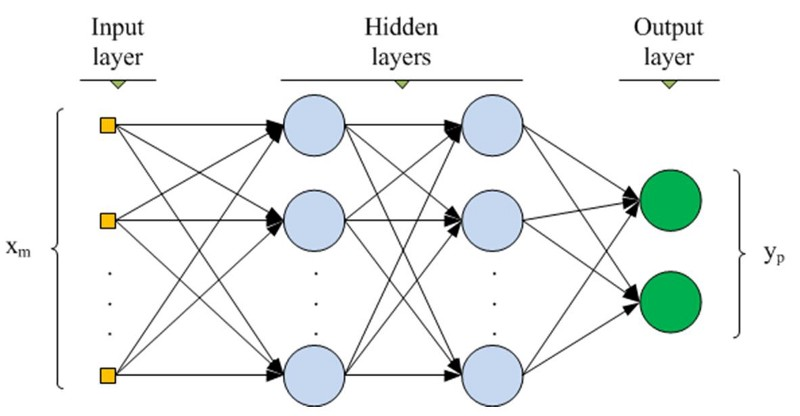
\includegraphics[width=\linewidth]{nn.jpeg}
  \caption{Deep Neural Network Classifier \cite{dnnc}}
  \label{fig:dnnc}
\end{figure}
\medskip \\
In our case, the input layer will be the feature column that generated by TensorFlow-Hub with module 'nnlm-en-dim128' as mentioned earlier. In general, the feature column is a neural network compatible representation of the input text. So, we do not need to manually choose and define features since we are applying a Deep Learning mechanism which has a well-defined feature representation of input. 
\medskip \\
Last but not least, the output layer will have 10 neurons as we have 10 classes (emojis), and each neuron represents how likely the input should be categorized as that class (should be using that emoji) accordingly. For each input text, we should pick the neuron that has the highest value in the output layer as our prediction to the input.

\section{Evaluation}
The evaluation matrices that we are going to use are accuracy and confusion matrix. They both generated by the methods of TensorFlow library. 
\begin{itemize}
\item Accuracy: A fraction of correct predictions. It represents how accurate of our model in predicting results by comparing that to the actual results.
\item Confusion Matrix: This matrix will have n rows and n columns, where n is the number of classes. The rows are represented predict class and the columns are represented actual class. 
\end{itemize}

\section{Analysis}
The system takes the development data as input to evaluate our Machine Learning model trained by the training data. The result is shown below.
\bigskip \\
\begin{tabular}{|c|c|c|}
      \hline
      Model & Accuracy \\
      \hline
      TensorFlow DNN & 0.5481749 \\
      \hline
\end{tabular}
\bigskip \\
Besides, we also used Gaussian Naive Bayes classifier from scikit-learn library to evaluate a Naive Bayes model which trained with the same training data with 'most100' feature. The model is evaluated to the same development data. The result is shown below.
\bigskip \\
\begin{tabular}{|c|c|c|}
      \hline
      Model & Accuracy \\
      \hline
      Naive Bayes & 0.2178692 \\
      \hline
\end{tabular}
\bigskip \\
From above result, we observed that the accuracy of Deep Learning model is surprisingly higher than the ordinary supervised

\section{Conclusion}
......

\bibliographystyle{plain}
\begin{thebibliography}{99}

\bibitem{nnlm} Bengio, Yoshua; Ducharme, Réjean; Vincent, Pascal; Jauvin, Christian {\em A Neural Probabilistic Language Model} 2003: Journal of Machine Learning Research, 3:1137-1155.

\bibitem{dnnc} Koehrsen, William {\em Deep Neural Network Classifier} 2017: Medium, https://medium.com/@williamkoehrsen/deep-neural-network-classifier-32c12ff46b6c

\end{thebibliography}
  
\end{document}
